\begin{solution}
	$\Rightarrow$
	\begin{center}
		\begin{tikzpicture}
			\tzcoor*(0, 0)(O){$O$}[l]
			\tzcoor(0:1.25)(P){$\d{r}$}[br]
			\tzcircle(O)(2)
			\tzline(O)(P){$r$}[mb]	
			\tzring[pattern=north east lines](O)(1.25)(O)(1.4)
		\end{tikzpicture}
	\end{center}
		\begin{align*}
			\intertext{We can use Gauss's law to find the electric field at $P$.}
			\intertext{We have to find out the total charge inside the point $P$.}
			q_i &= \int_{0}^{r} \uprho \d{V}\\
			 	&= \int_0^r \uprho_0 \left(\dfrac{3}{4}-\dfrac{r}{R}\right)4\pi r^2 \d{r}\\
				&= \pi\uprho_0\int_{0}^{r} \left(3r^2 - \dfrac{4r^3}{R} \right) \d{r}\\
				&= \pi\uprho_0\left[r^3 - \dfrac{r^4}{R}\right]_0^r\\
				&= \pi\uprho_0\left(r^3 - \dfrac{r^4}{R}\right)\\
			\intertext{Apply the Gauss's law.}
			\oint \vec{E}\cdot\d{\vec{A}} &= \dfrac{q_i}{\epsilon_0}\\
			\Rightarrow E\cdot 4\pi r^2 &= \dfrac{\pi\uprho_0\left(r^3 - \dfrac{r^4}{R}\right)}{\epsilon_0}\\
			\Rightarrow E &= \dfrac{\uprho_0 r}{4\epsilon_0}\left(1-\dfrac{r}{R}\right)
		\end{align*}
	\end{solution}